\begin{questions}

\question{Using {\bf weno3.m}, investigate the effects of the CFL
factor $r$ on the solution of the Riemann problem
\begin{displaymath}
	\rho_L = 1,~ u_L = 0,~ p_L = 1 ;~~~
	\rho_R = 0.125,~ u_R = 0,~ p_R = 0.1
\end{displaymath}
with $\gamma$ = 1.4.  Take 200 $\Delta x$ and CFL factor $r$ = 0.1,
0.5, 0.9.  Turn in the Density plots (computed vs.\ exact solution) at
time $t = 0.2$ for each of three cases.  Briefly discuss your results.}
\begin{solution}
In the following figures we can see the solution to the problem compared to the exact solution. Since in all cases the method is stable, the solutions are mostly undistinguishible. However, the smaller the $CFL$ factor, the longer it takes the simulation to finish.
\begin{figure}[H]
\centering     %%% not \center
{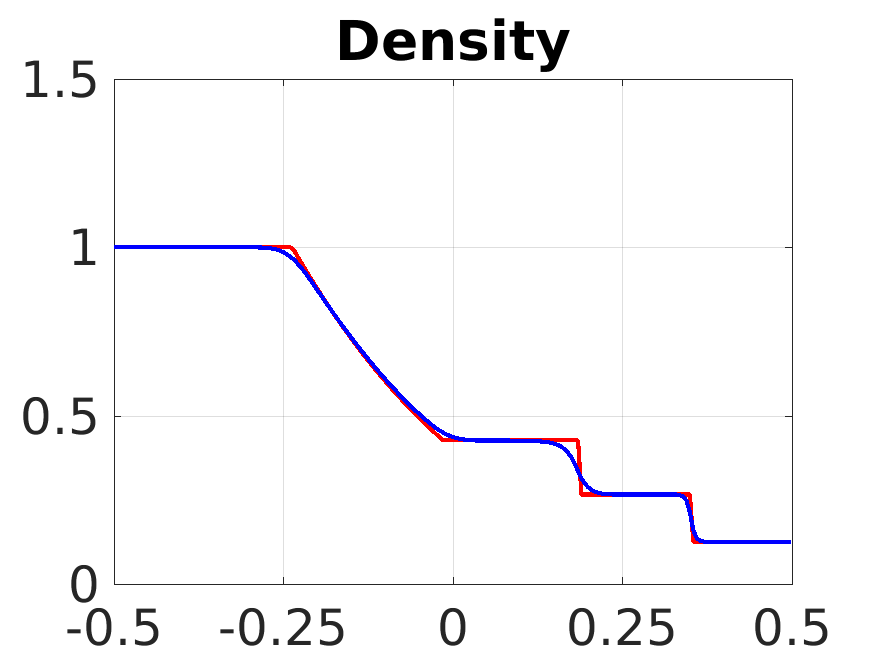
\includegraphics[scale=0.5]{density_r01.png}}
\caption{$CFL= 0.1$.}
\end{figure}
\begin{figure}[H]
\centering     %%% not \center
{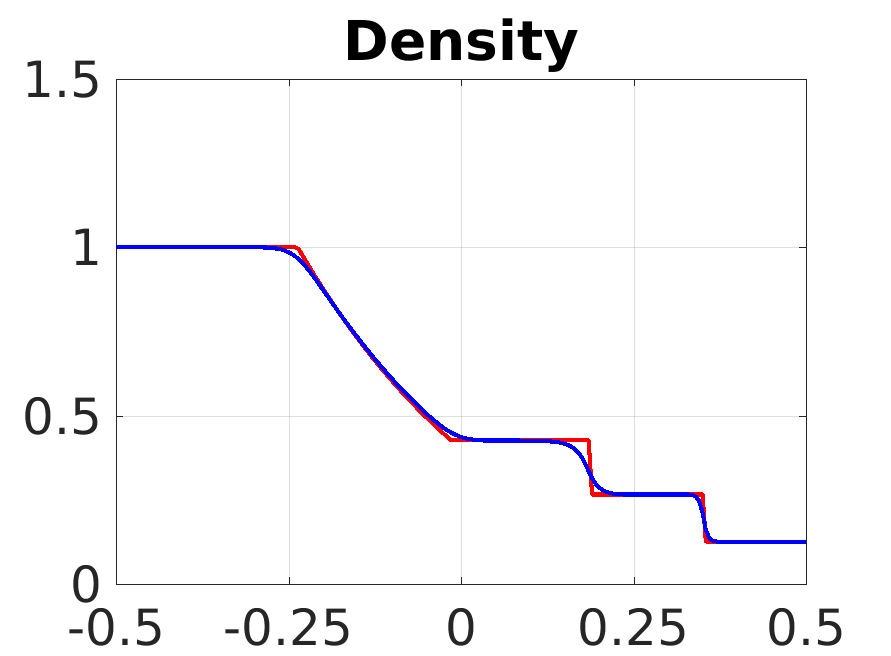
\includegraphics[scale=0.5]{density_r05.png}}
\caption{$CFL= 0.5$.}
\end{figure}
\begin{figure}[H]
\centering     %%% not \center
{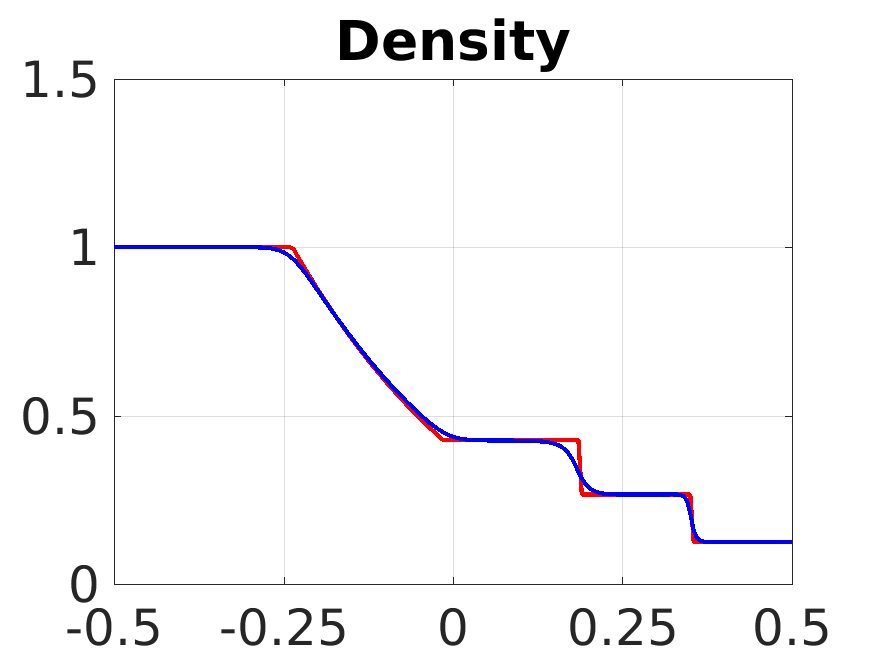
\includegraphics[scale=0.5]{density_r09.png}}
\caption{$CFL= 0.9$.}
\end{figure}
\end{solution}
\end{questions}
